\section{V14}
\subsection{Spezielle Eigenschaften des NVIC}\label{NVIC}
\subsubsection{Tail Chaining}
Wenn eine Exception auftritt während bereits eine ander Exception-Behandlunf mit gleicher oder höherer Priotität läuft, so wird die neue Exception hintenangestellt. Nach Abschluss des laufenden Exception Handlers, kann die CPU sofort den neuen Exception Request behandeln

\subsubsection{Late arrival}
Wenn der Prozessor einen auftretenden Exceptionrequest akzeptiert, dann startet er die Stacking-Sequenz. Kommt während dem stacking eine weitere Exception mit höherer Priorität hinzu, so kann diese Late-Arrival-Exception noch bevorzugt behandelt werden.

\subsubsection{POP Preemption}
Diese Funktion stellt gewissermassen eine Umkehrung des Late-Arribals dar. Wenn eine Exception Request während dem Unstacking auftritt, so wird das Unstacking abgebrochen, und sofort VectorFetch und Instruction Fetch für den neuen Request durchgeführt. $\rightarrow$ Geschwindigkeitsoptimierung\\

\subsection{Cortex-M3 Exceptions und Priority-Levels}
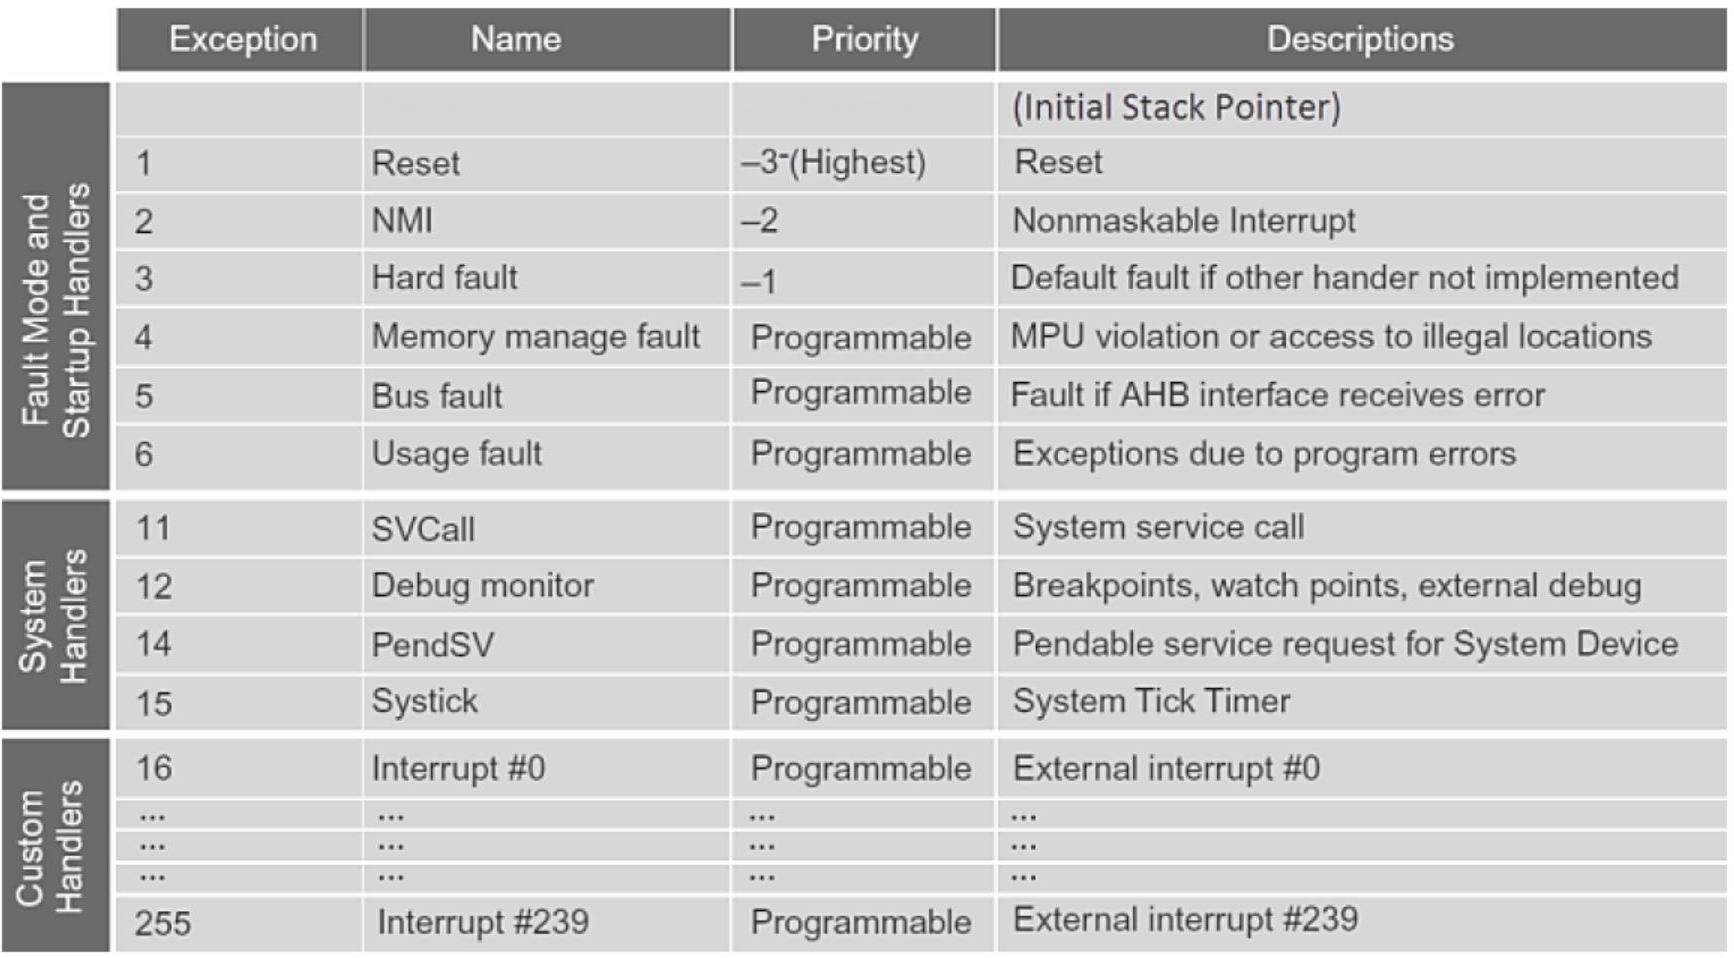
\includegraphics[width=1\linewidth]{images/NVICExcp1} 